\section{Algorithm}

\begin{figure}[h]
  \centering
  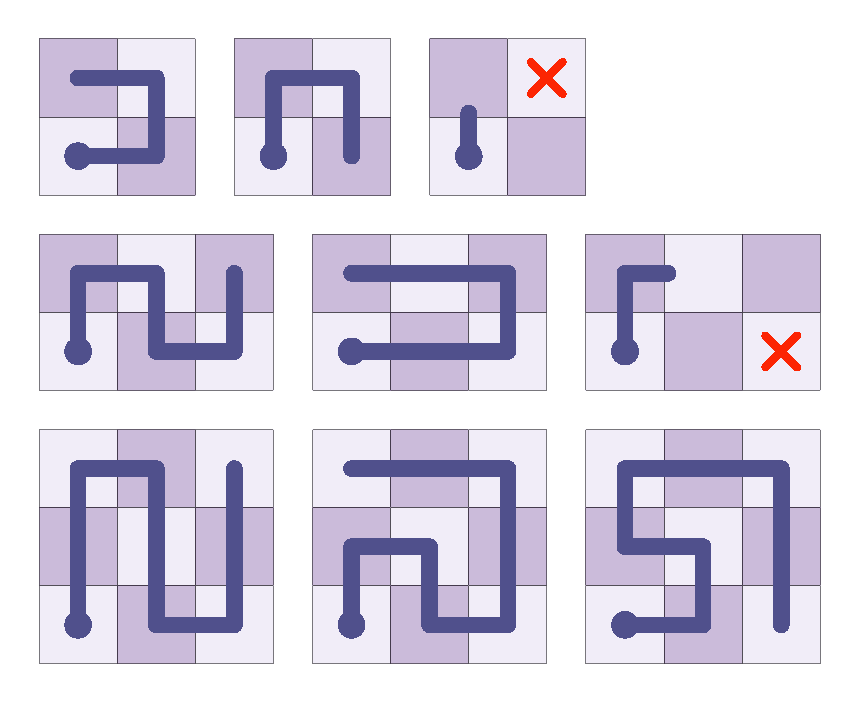
\includegraphics[width=\linewidth]{simple_hampath.pdf}
  \caption{ Illustrative examples of Hamiltonian paths height/width that are even/even, even/odd and odd/odd, respectively,
            when starting from the lower left hand corner }
  \label{fig:exampleHampath}
\end{figure}


\begin{figure}[h]
  \centering
  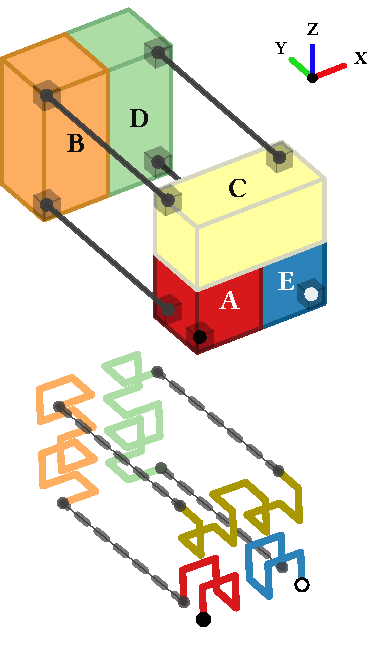
\includegraphics[width=\linewidth]{gilbert3d_explode.pdf}
  \caption{ The J-split subdivision, representing the main subdivision of the build recursion for the 3D Gilbert curve case }
  \label{fig:gilbert3DJSplit}
\end{figure}


\begin{figure*}[ht]
  \centering
  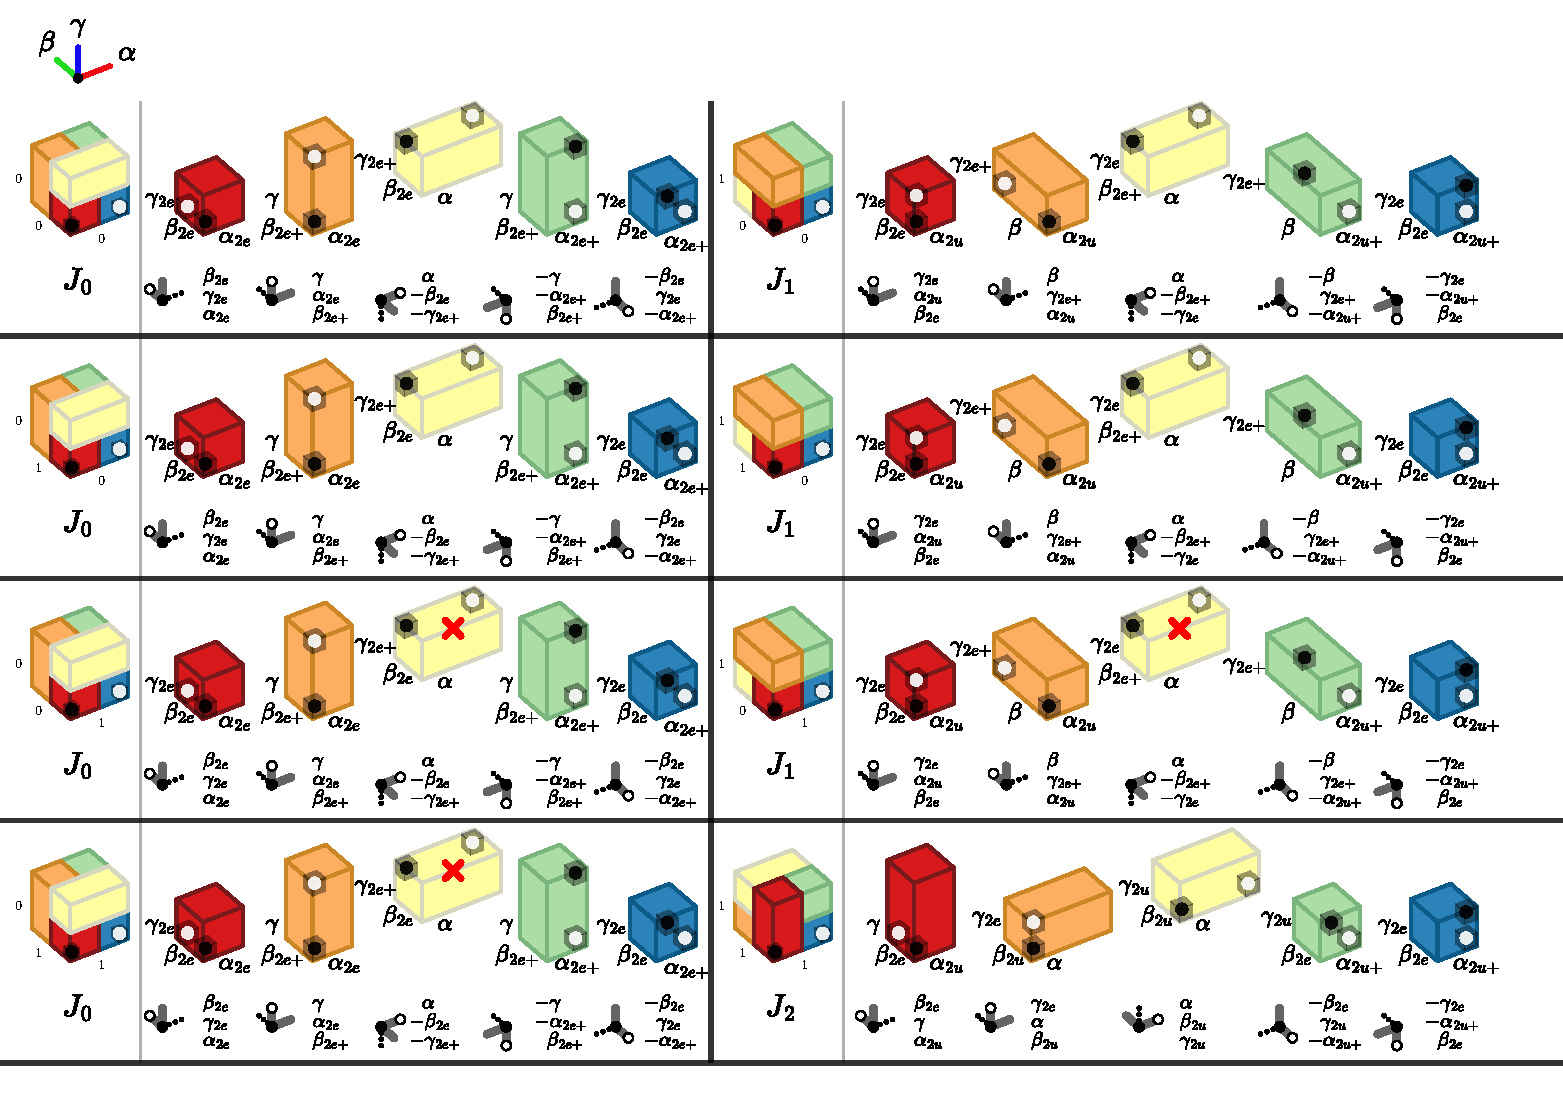
\includegraphics[width=\textwidth]{gilbert3d_case.pdf}
  \caption{ Bulk recursion J-split atlas for the 3D Gilbert algorithm }
  \label{fig:gilbert3DCase}
\end{figure*}



